\documentclass[letterpaper]{article}
\usepackage[margin=1in]{geometry}
\usepackage[utf8]{inputenc}
\usepackage{amsmath}
\usepackage{amssymb}
\usepackage{mathrsfs} %for math script%
\usepackage{graphicx}
\usepackage{float}
%\usepackage{flafter}
%\usepackage{afterpage}
\usepackage{indentfirst}
\usepackage{hyperref}
\graphicspath{{figures/}}
\setlength{\parindent}{0pt}

\newcommand{\Dt}{\Delta t}
\newcommand{\Dx}{\Delta x}

\begin{document}

\section{ARZ model}

Consider the full nonlinear ARZ model without relaxation \cite{AR, Z}:
\begin{align} 
\rho_t + (\rho v)_x &= 0, \label{ARZ1} \\
(v - V(\rho))_t + v(v - V(\rho))_x &=0. \label{ARZ2}
\end{align}

\section{Numerical schemes}

\subsection{Godunov}

The Godunov scheme requires a Riemann solver. To apply this scheme we first write the system in conservation form. The model is \cite{GodunovARZ}:
\begin{equation} \label{eq:consv}
U_t + [F(U)]_x = 0,
\end{equation}
with conserved variables $U = \begin{pmatrix} \rho \\ y \end{pmatrix}$ and flux vector $F(U) = \begin{pmatrix} y + \rho V(\rho) \\ \dfrac{y^2}{\rho} + y V(\rho) \end{pmatrix}$.

The scheme is 
\begin{equation}
U^{n+1}_j = U^n_j - \dfrac{k}{h}\left[F(u^*(U^n_j, \, U^n_{j+1})) - F(u^*(U^n_{j-1}, \, U^n_j))\right],
\end{equation}
where $u^*(U^n_j, \, U^n_{j+1})$ is the solution to the Riemann problem with initial data $U^n_j$ and $U^n_{j+1}$. The Riemann problem solution is discussed in \cite{GodunovARZ}.

\subsection{Lax-Friedrichs}
The Lax-Friedrichs scheme can be applied to equations in the form of \eqref{eq:consv} as well, but a Riemann solver is not needed. The partial derivatives are approximated using a forward difference in time and central difference in space, and $U^n_j$ is replaced with its spatial average. The scheme is:
\begin{equation}
U^{n+1}_j = \frac{1}{2}[U^n_{j+1} - U^n_{j-1}] - \dfrac{\Dt}{2 \Dx}[F(U^n_{j+1}) - F(U^n_{j-1})].
\end{equation}

This method is first-order accurate and very dissipative \cite{LeVequetext}. The stencil for this method is shown in Figure 
\ref{fig:stencil_laxfried}. \\

\begin{figure}[H]
\centering
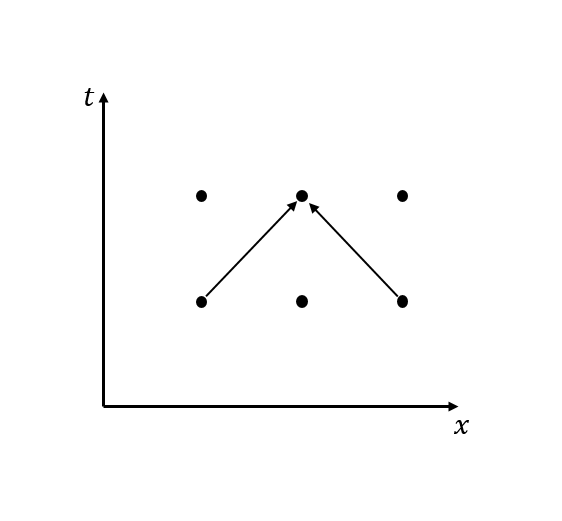
\includegraphics[trim = 10mm 20mm 10mm 15mm, width=0.3\textwidth]{Laxfried.png}
\caption{Stencil for Lax-Friedrichs method.}
\label{fig:stencil_laxfried}
\end{figure}


\subsection{Lax-Wendroff}
We look at a higher-order scheme with less numerical dissipation. For nonlinear conservation laws, the Lax-Wendroff scheme is: 
\begin{align}
U^{n+1}_j = U^n_j &- \dfrac{\Dt}{2 \Dx}[F(U^n_{j+1}) - F(U^n_{j-1})] + \dfrac{(\Dt)^2}{2 (\Dx)^2}[A_{j+1/2}(F(U^n_{j+1}) \notag \\ 
&- F(U^n_j)) - A_{j-1/2}(F(U^n_j)- F(U^n_{j-1}))]
\end{align}
where $A_{j\pm 1/2}$ is the Jacobian matrix $F'(\cdot)$ evaluated at $\frac{1}{2}(U^n_j + U^n_{j\pm1})$. Evaluating the Jacobian matrix makes this method more expensive to use so Richtmyer proposed a two-step procedure to avoid using $A$. In the first step $u(x,t)$ is calculated at half time and space steps. In the second step these values are used to compute the solution at the next time step. 

Richtmyer's two-step Lax-Wendroff method is: 

First step:
\begin{align}
U^{n+1/2}_{j+1/2} &= \dfrac{1}{2}(U^n_{j+1} + U^n_j - \dfrac{\Dt}{2 \Dx} [F(U^n_{j+1} - F(U^n_j)] \\
U^{n+1/2}_{j+1/2} &= \dfrac{1}{2}(U^n_j + U^n_{j-1} - \dfrac{\Dt}{2 \Dx} [F(U^n_j - F(U^n_{j-1})]
\end{align}
Second step:
\begin{equation}
U^{n+1}_j = U^n_j - \dfrac{\Dt}{\Dx}[F(U^{n+1/2}_{j+1/2}) - F(U^{n-1/2}_{j-1/2})]
\end{equation}

This method is second-order accurate and less dissipative than the Lax-Friedrichs method.  However, as the Lax-Wendroff method does not preserve monotonicity, it produces oscillations near discontinuities \cite{LeVequetext}. 

The stencil for this method is shown in Figure 
\ref{fig:stencil_laxwend}. \\

\begin{figure}[H]
\centering
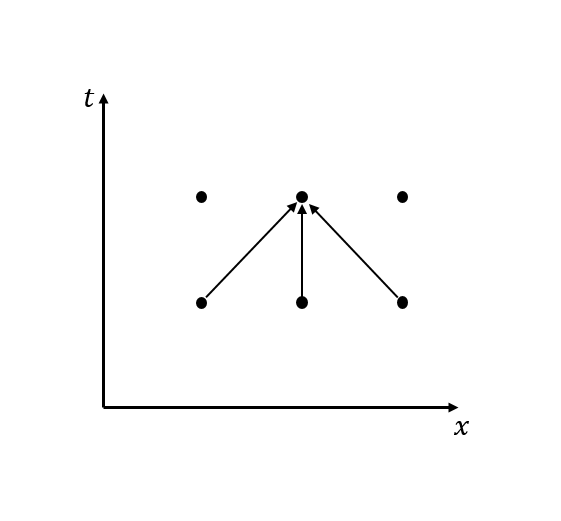
\includegraphics[trim = 10mm 20mm 10mm 15mm, width=0.3\textwidth]{Laxwend.png}
\caption{Stencil for Lax-Wendroff method.}
\label{fig:stencil_laxwend}
\end{figure}


\subsection{ENO and WENO}

The ENO (essentially non-oscillatory) schemes were developed by Harten, Engquist, Osher, and Chakravarthy to solve the problem of finding highe-order schemes that do not produce oscillations near discontinuities. The idea is to use a high-degree polynomial interpolate the solution $U$ then compute $U_x$. The stencil is chosen depending on the upwind direction, then points are added so that the interpolant has the least oscillation. \\

The WENO (weighted ENO) scheme, introduced by Liu, Osher, and Chan \cite{WENO}, uses a convex combination approach rather than picking the smoothest stencil in order to achieve the ENO property. 



\bibliographystyle{ieeetr}
\bibliography{mybibfile}


\end{document}